\chapter{Raíces de ecuaciones}

\begin{chapquote}{Lozano, 2024}
    ``No se preocupen si no entienden esto, yo tampoco.''
\end{chapquote}


\section{Antecedentes matemáticos}

En general, existen dos tipos de funciones matemáticas:

\begin{definition}[Función algebraica]
	En el caso de una variable, se dice que una función \(f(x)\) es
	algebraica si se expresa de la siguiente manera:

	\[
		f_n y^n + f_{n-1} y^{n-1} + ... + f_1 y + f_0 = 0
	\]

	Donde cada \(f_i (i = 0, 1, ..., n)\) es un polinomio de la forma:

	\[
		f_i = a_{in} X^i + a_{i(n-1)} x^{i-1} + ... + a_{i1} x + a_{i0}
	\]
\end{definition}

\begin{definition}[Función trascendental]
	Es aquella que no es algebraica.
\end{definition}

\begin{eg}
	Las funciones trigonométricas, exponenciales, logarítmicas, las de
	Bessel, Jacobi, Mittag Leffler, entre muchas otras, son trascendentes.
	Por ejemplo, el logaritmo natural se puede definir así:

	\[
		\boxed{\ln(x) = \int_1^x \frac{d \tau}{\tau}, x > 0}
	\]

\end{eg}

Solucionar ecuaciones algebraicas o trascendentes implica el uso de dos tipos de
métodos numéricos: los métodos cerrados y los métodos abiertos. Los primeros
utilizan dos valores que encierran a la raíz, mientras que los segundos sólo
uno.

\section{Métodos cerrados}

Este tipo de métodos aprovecha el cambio de signo que se presenta cuando una
función pasa a través del eje de las abscisas para detectar una raíz. Se les
conoce por ese nombre porque necesitan un intervalo cerrado que contenga a la
raíz. Un método cerrado muy sencillo es el \textbf{método de bisección}.

\subsection{Método de bisección}

En general, si $f(x)$ es una función real y continua en el intervalo $[x_l,
x_u]$ y además $f(x_l)$ y $f(x_u)$ tienen signos opuestos, \textit{i.e.}
$f(x_l) f(xu) < 0$, se sabe que \textbf{existe al menos una raíz entre $x_l$ y
$x_u$}.

El método consiste en dividir el intervalo original a la mitad (hacer una
bisección) y descartar aquella mitad donde no haya raíces. El proceso se repite
tantas veces como sea necesario hasta que el intervalo sea, en términos
prácticos, un sólo punto: la raíz buscada. Es un \textit{binary search de
raíces}.

\subsubsection{Algoritmo para el método de bisección}

\begin{enumerate}
	
	\item Elija el intervalo que encierra la raíz, es decir, $[x_l, x_u]$.
		Verifique que $f(x_l)f(x_u) < 0$.

	\item Obtenga la aproximación de la raíz con $x_r \approx \frac{x_l +
		x_u}{2}$

	\item Para determinar el nuevo sub-intervalo, evalúe:
		\begin{itemize}
			\item Si $f(x_l)f(x_r) < 0$, entonces la raíz debe
				encontrarse en el intervalo $[x_l, x_r]$. El
				algoritmo se seguirá ejecutando de manera
				recursiva.
			\item Si $f(x_l)f(x_r) > 0$, entonces la raíz debe
				encontrarse en el intervalo $[x_r, x_u]$. El
				algoritmo se seguirá ejecutando de manera
				recursiva.

			\item Si $f(x_l) f(x_r) = 0$, entonces $x_r$ es la raíz
				buscada, o
				\[
					\varepsilon_a < \varepsilon_s
				\]

				Donde $\varepsilon_a$ es el \textbf{error relativo
				aproximado} y $\varepsilon_s$ es la
				\textbf{tolerancia} (\textit{sufferance})
				prefijada.
		\end{itemize}
\end{enumerate}

Pocas veces se conoce a priori el valor de la raíz real. Por ello, se
debe definir una aproximación mediante el error relativo aproximado:

\[
	\varepsilon_a = \left| \frac{x_i - x_{i-1}}{x_i} \right| \times 100\%
\]

Una fórmula comúnmente usada para la elegir una tolerancia en cálculos numéricos
donde se quiere garantizar un número $n$ de cifras significativas es la
siguiente:

\[
	\varepsilon_s = 0.5 \times 10^{2-n} \%
\]

\begin{ex}

	Encuentre la raíz de la ecuación \ref{primer-problema}:

	\[
		x^2 - 4 - sin(x) = 0
	\]

	\begin{solution}
		Tomando $f(x) = x^2 - 4 - sin(x)$, uno puede utilizar un
		lenguaje de programación para implementarel algoritmo ya
		descrito.

		\lstinputlisting[language=Fortran, caption=Implementación del
		método de bisección en Fotran.,
		label={lst:bisect-fortran}]{./programas/metodo-biseccion/biseccion.f90}

		\lstinputlisting[language=Go, caption=Implementación del
		método de bisección en Go.,
		label={lst:bisect-go}]{./programas/metodo-biseccion/biseccion.go}
	\end{solution}
	
\end{ex}

\subsection{Método de la falsa posición}

Como se vio anteriormente, el método de bisección es bastante útil para hallar
raíces de ecuaciones el cual únicamente usa fuerza bruta. \textbf{No obstante,
su tiempo de cómputo en comparación de otros métodos es alto}. Una alternativa a
tal método es el de la \textbf{falsa posición}, el cual tiene la siguiente ecuación
recursiva:

\[
	x_r = x_u - \frac{f(x_u) (x_l-x_u)}{f(x_l) - f(x_u)}
\]

\subsubsection{Algoritmo para el método de la falsa posición}

\begin{enumerate}
	
	\item Elija el intervalo que encierra la raíz, es decir, $[x_l, x_u]$.
		Verifique que $f(x_l)f(x_u) < 0$.

	\item Obtenga la aproximación de la raíz con:
		\begin{equation*}
			x_r = x_u - \frac{f(x_u)(x_l-x_u)}{f(x_l) - f(x_u)}
		\end{equation*}

	\item Para determinar el nuevo sub-intervalo, evalúe:
		\begin{itemize}
			\item Si $f(x_l)f(x_r) < 0$, entonces la raíz debe
				encontrarse en el intervalo $[x_l, x_r]$. El
				algoritmo se seguirá ejecutando de manera
				recursiva.
			\item Si $f(x_l)f(x_r) > 0$, entonces la raíz debe
				encontrarse en el intervalo $[x_r, x_u]$. El
				algoritmo se seguirá ejecutando de manera
				recursiva.

			\item Si $f(x_l) f(x_r) = 0$, entonces $x_r$ es la raíz
				buscada, o
				\[
					\varepsilon_a < \varepsilon_s
				\]

				Donde $\varepsilon_a$ es el \textbf{error relativo
				aproximado} y $\varepsilon_s$ es la
				\textbf{tolerancia} (\textit{sufferance})
				prefijada.
		\end{itemize}
\end{enumerate}

\begin{ex}
	Resuelva el ejercicio anterior mediante el método de falsa posición
	
	\begin{solution}

		Puede implementarse el algoritmo descrito anteriormente en un
		programa de computadora de la siguiente manera:

		\lstinputlisting[language=Fortran, caption=Implementación del
		método de la falsa posición en Fotran.,
		label={lst:false-fortran}]{./programas/metodo-falsa-posicion/falsa.f90}

		\lstinputlisting[language=Go, caption=Implementación del
		método de la falsa posición en Go.,
		label={lst:false-go}]{./programas/metodo-falsa-posicion/falsa.go}
	\end{solution}
\end{ex}

Obvserve que el método de la falsa posición, converge, por lo general, más
rápido que el método de bisección. Lo anterior se debe a que, dependiendo de la
naturaleza de $f(x)$, en ocasiones se descarta el intervalo más grande.


\section{Métodos abiertos}

Mientras que los métodos cerrados garantizan la convergencia a una raíz, este
tipo de métodos depende sensiblemente de las condiciones iniciales para su
ejecución, pues divergen con facilidad.

\subsection{Método de punto fijo (o función contraída)}

Este es uno de los métodos más simples. Si se quiere encontrar la raíz de una
función $f(x)$ donde se puede despejar alguna $x$, se puede obtener una
relación de recurrencia para calcular las raíces:

\begin{equation}\label{pape}
	f(x) = 0 \implies \boxed{x = g(x)}
\end{equation}

Si, eligiendo un dominio $D$ donde exista la raíz,

\[
	\left| g'(x) \right| < 1 \land x \in D
\]

puede transformarse \ref{pape} en una relación de recurrencia:

\[
	x_{i+1} = g(x_i)
\]

\begin{ex}
	Use el método de iteración de punto fijo para encontrar las raíces de la
	función:

	\[
		e^{-x} - x = 0
	\]

	\begin{solution}
		Puede definirse lo siguiente:

		\[
			f(x) = e^{-x} - x = 0 \implies x = e^{-x} = g(x)
		\]

		Teniendo en cuenta la gráfica de la función, la raíz es
		aproximadamente $x_r \approx 0.6$, por lo que pude verificarse
		que la derivada tiene magnitud menor a uno:

		\begin{figure}
			\centering
			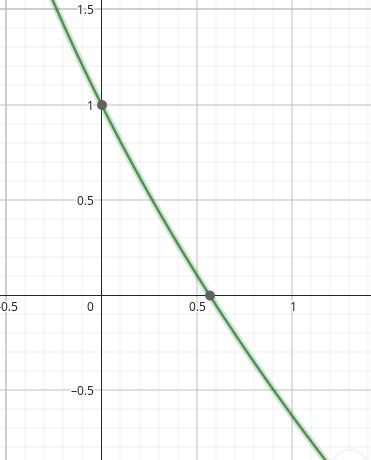
\includegraphics[height=2in]{img/punto-fijo-img.png}
			\caption{Función $f(x) = e^{-x} - x$}
		\end{figure}

		\[
			|g'(x)| = |-e^{-x}| e^{-x} = \frac{1}{e^x} < 1 \forall x \in (0,
			\infty)
		\]

		Como la condición se satisface, puede escribirse la ecuación de
		recurrencia

		\[
			x_{i+1} = e^{-x_i}
		\]

		Si se toma una $x_0 = 1$ y se empiezan a obtener resultados de
		manera iterativa, $x \rightarrow 0.5671432904$

		% importar tabla
	\end{solution}
\end{ex}

El método tiene este nombre debido a su interpretación geométrica. El valor
inicial $x_0 = 1$, con una vertical toca a $g(x)$, después una horizontal toca a
la función identidad nuevamente. El proceso se repite de manera que se forma una
espiral de donde surge el nombre ``función contraída''

\begin{ex}
	La siguiente ecuación puede resolverse vara valores de $r \in [0,4]$,
	donde $r$ representa la taza de crecimiento poblacional:

	\[
		x - rx(1 - x) = 0
	\]

	Donde, aplicando el método de punto fijo se obtiene la relación:

	\[
		x_{n+1} = r x_n (1 - x_n)
	\]

	Esta ecuación es conocida como la \textbf{ecuación logística}, que tiene
	su origen en la dinámica de poblaciones, los términos son:

	\begin{align*}
		rx_n &= \text{taza de nacimientos} \\
		(1 - x_n) &= \text{taza de mortandad}
	\end{align*}

	\lstinputlisting[language=Fortran, caption=Código para obtener el
	diagrama de bifurcación mediante el método de punto fijo en Fotran.,
	label={lst:bifurc-fortran}]{./programas/bifurcacion/bifurcacion-logistica.f90}

	\begin{figure}
		\centering
		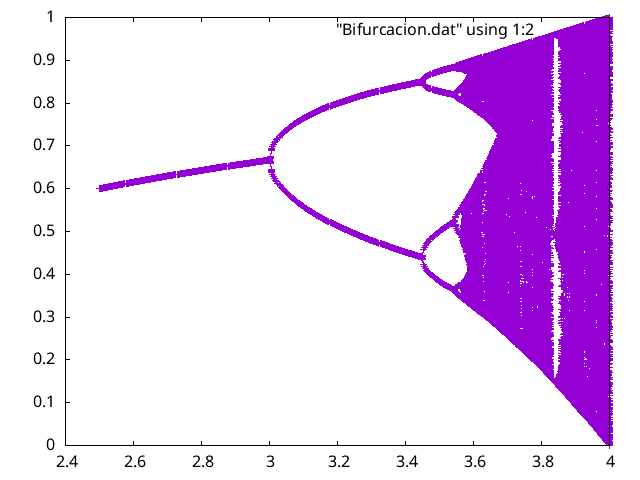
\includegraphics[width=1.0\textwidth]{programas/bifurcacion/bifurcacion.png}
		\caption{Diagrama de bifurcación creado con el programa de
		Fortran.}
	\end{figure}
\end{ex}

\subsection{Método de Newton-Raphson}

El método de Newton-Raphson es popular debido a la facilidad con la que puede
ser implementado, así como por sun velocidad de convergencia cuando se le da un
valor inicial adecuado. El método consiste en el trazo de una recta tangente
desde el punto $(x, f(x))$ e ir acercándose progresivamente a la raíz $x_r$.

El esquema de Newton-Raphson se obtiene a partir de la serie de Taylor truncada
a términos de primer orden,

\[
	f(x_{x+1}) \approx f(x_n) + f'(x_n)(x_{n+1} - x_n)
\]

Como $x_{n+1}$ es una raíz, se deduce que $f(x_{n+1}) \approx 0$ y a partir de
ahí se obtiene la siguiente relación de recurrencia

\begin{equation}\label{eqn:newton}
	x_{n+1} = x_n - \frac{f(x_n)}{f'(x_n)}
\end{equation}

\begin{ex}
	Obtenga la raíz de la siguiente ecuación,

	\[
		f(x) = x^3 + x^2 + \ln(x) + 2 \cos(x) = 0
	\]

	\begin{solution}

		Es buena idea obtener la gráfica de la función para ppoder
		visualizar las intersecciones y elegir un mejor valor inicial.

		La derivada es 

		\[
			f'(x) = 3x^2 + 2x + \frac{1}{x} - 2 \sin(x)
		\]

		Para encontrar el esquema correspndiente de Newton-Raphson,
		puede usarse el siguiente esquema:

		\begin{align*}
			x_{n+1} &= x_n - \frac{f(x_n)}{f'(x_n)} \\
				&= x_n - \frac{x^3 + x^2 + \ln(x) + 2
				\cos(x)}{3x^2 + 2x + \frac{1}{x} - 2 \sin(x)}
		\end{align*}

		Conociendo que la raíz está cerca de 0.15, puede utilizarse una
		calculadora para empezar estas iteraciones. El resultado es:

		\[
			\boxed{r \approx 0.1349}
		\]

	\end{solution}

\end{ex}

\begin{ex}
	Encuentre la raíz real del polinomio 

	\[
		18.95x^3 + 5x^2  + 0.33x + 1 = 0
	\]

	\begin{solution}
		Se aplica la fórmula \ref{eqn:newton} para aplicar el método de
		Newton-Raphson

		\begin{align*}
			x_{n+1} &= x_n - \frac{f(x_n)}{f'(x_n)} \\
				&= x_n - \frac{18.95x_n^3 + 5x_n^2 + 0.33x_n +
				1}{3(18.95)x_n^2 + 10x_n + 0.33}
		\end{align*}

		Tomando como punto inicial a \(x_0 = -0.5 \), el valor de la raíz
		llega a:

		\[
			\boxed{x_{r_1} \approx -0.4677830945}
		\]

		Conociéndose esta raíz, puede utilizarse división sintética para
		crear una aproximación de polinomio de segundo grado cuyas
		raíces pueden ser calculadas con la fórmula general. A este
		proceso se le conoce como \textit{deflación polinomial}:

		\begin{center}
			\begin{tabular}{ c | c c c c }
				& 18.95 & 5 & 0.33 & 1 \\
			        0.467731 & & -8.8644896 & 1.80774292 & -1 \\
			 \hline
				 & 18.95 & -3.8644896 & 2.13774292 & 0
			\end{tabular}
		\end{center}

		Se obtiene el polinomio 

		\[
			18.95x^2 - 3.8644896x + 2.13774292
		\]

		Que puede solucionarse con la fórmula general, obteniendo las
		raíces faltantes:

		\begin{align*}
			x_{r_1} &= -0.467783 \\
			x_{r_2} &= 0.1019 + 0.32001 i \\
			x_{r_3} &= 0.1019 - 0.32001 i 
		\end{align*}
	\end{solution}

	% Incertidumbres, integrales con series de taylor, bisección, punto fijo,
	% newton-raphson
\end{ex}

\subsection{Método de la secante}

El método de Newton-Raphson que se describió anteriormente y formulado por la
ecuación \ref{eqn:newton} emplea una derivada en el denominador. Si la función
cuyas raíces se quieren encontrar es dificil de derivar, puede que utilizar este
método no sea ideal. En estos casos, se recurre a modificar el método para
sustituir la derivada por un esquema numérico en diferencias finitas centradas:

\[
	f'(x_i) \approx \frac{f(x_i) - f(x_{i-1})}{x_i - x_{i-1}}
\]
